\documentclass[border=10pt]{standalone}
\usepackage{pgfplots}
\pgfplotsset{compat=1.18}
\begin{document}
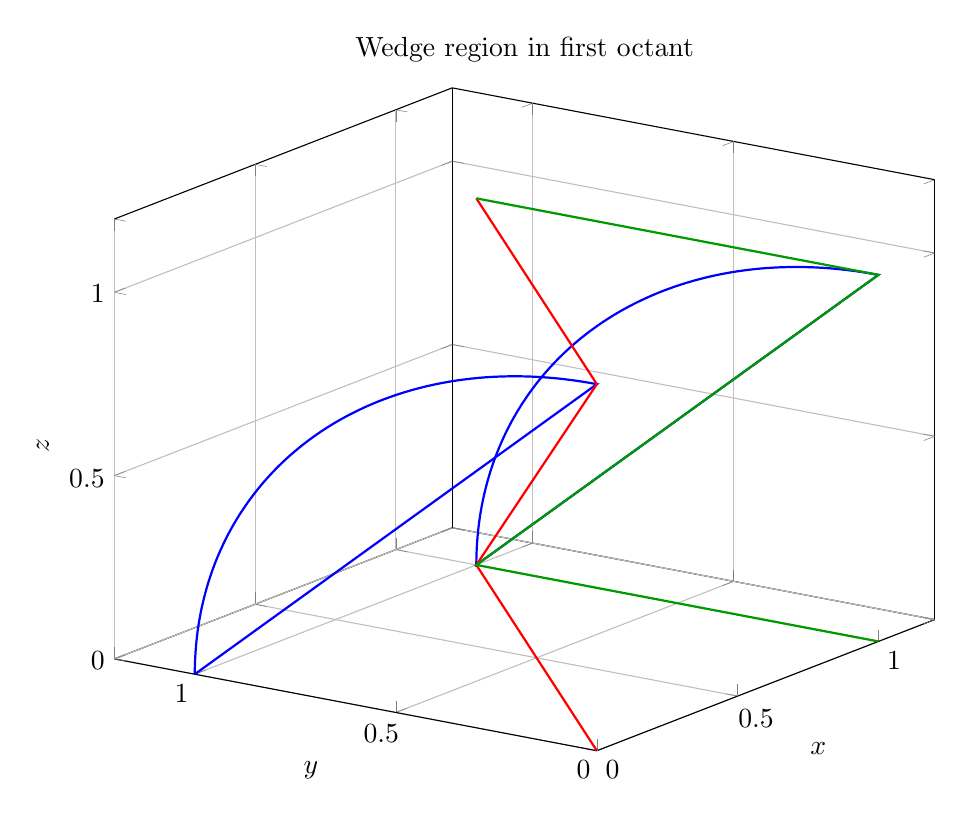
\begin{tikzpicture}
\begin{axis}[
    view={-55}{20},
    xlabel={$x$}, ylabel={$y$}, zlabel={$z$},
    xmin=0, xmax=1.2, ymin=0, ymax=1.2, zmin=0, zmax=1.2,
    xtick={0,0.5,1}, ytick={0,0.5,1}, ztick={0,0.5,1},
    title={Wedge region in first octant},
    grid=both,
    width=12cm, height=10cm,
]

% Cylinder boundary
\addplot3[blue, thick, samples=80, domain=0:90, variable=\t]
    ({0}, {cos(\t)}, {sin(\t)});
\addplot3[blue, thick, samples=80, domain=0:90, variable=\t]
    ({1}, {cos(\t)}, {sin(\t)});

% Plane y = x
\addplot3[red, thick, samples=2, domain=0:1, y domain=0:1]
    ({x}, {x}, {y});

% Plane x = 1
\addplot3[green!60!black, thick, samples=2, domain=0:1, y domain=0:1]
    ({1}, {x}, {y});

\end{axis}
\end{tikzpicture}
\end{document}